\section{Cyanobacteria}
\epigraph{The following sections were written by Malin Eriksson and Maxence Holtz}{\textit{iGEM Aboa \& Toulouse\_INSA-UPS 2021}}
\subsection{Overview}
The ability to transform an organism is essential in any synthetic biology project. Exogenous DNA can be introduced into cyanobacteria mainly in three different ways, either for the chromosomic integration of transgene expression cassettes through homologous recombination or for the transfer of stably replicable plasmids. These approaches are natural transformation, electroporation, and conjugation. The method of choice depends on many factors, including cyanobacterial strain and available equipment.

\subsection{Natural transformation}
Many cyanobacterial species are naturally competent, meaning that they readily take up exogenous DNA from their environment . Cyanobacteria can integrate the exogenous DNA into their genome through homologous recombination or maintain circular heterologous DNA elements in the presence of a proper replication origin. Natural competency has not been studied in as much detail in cyanobacteria as it has in many heterotrophic organisms \parencite{Schirmacher2020}. Thus, many aspects relating to the exact mechanism of DNA uptake are still somewhat unclear. The two most discussed hypotheses for the advantages of natural competence are DNA-for-diversity and DNA-for-food. The DNA-for-diversity hypothesis suggests that the benefit of natural competence is the ability to obtain new features, whereas the DNA-for-food hypothesis states that DNA uptake is nutriciously important \parencite{Schirmacher2020}. \\ \\
Naturally competent cyanobacteria provide an efficient and easy-to-use method for the introduction of foreign DNA into the cells. In brief, this transformation method only requires the DNA that is to be taken up and a cyanobacterial liquid culture to which it will be mixed into. Thus, no particular equipment or reagents are necessary besides those found in a cyanobacteria culture laboratory and preparation time is minimal. Protocols for natural transformation tend to vary between research groups, and also may need some adaptations from one species to another, meaning that no consensus has been reached. Optimization attempts have usually circled around changing parameters such as incubation time, light conditions during incubation, DNA concentration, cyanobacterial growth phase, and plating style \parencite{Zhang2007}. \\ \\
Relying on the natural competence of cyanobacteria is, however, not always possible, as only certain cyanobacterial strains carry this trait. Cyanobacteria within the \textit{Synechocystis} and some within the  \textit{Synechococcus} genus are naturally competent \parencite{Schirmacher2020}. These are among the most well-studied and used cyanobacteria in research, but if the project plan involves utilization of other species, another transformation method could be vital. It is important to emphasize that certain species, such as spirulina (\textit{Arthrospira platensis}) that is widely used as a nutritional protein source, have not been successfully transformed to date. 

\subsection{Conjugation}
Conjugal transfer of DNA between bacterial cells is a well-described process and has been used previously to engineer cyanobacterial species, particularly those that are not naturally competent, such as \textit{S. elongatus} UTEX 2973 \parencite{Elhai1988} \parencite{Yu2015}. To obtain stable conjugal transfer it is necessary (1) conjugal contacts to be made, (2) the transferred DNA to escape restriction or degradation, and (3) the transferred DNA to replicate autonomously or integrate into one of the replicons of the recipient \parencite{Elhai1988} \parencite{Gale2019}. \\ \\
In brief, cyanobacterial cultures are incubated in the presence of two different E. coli strains called respectively the conjugal strain and the helper strain. Note that in some variations of this protocol, only one E. coli strain carries all the plasmids. The helper strain carries two plasmids: the vector to be transferred to the cyanobacteria called cargo vector and a helper plasmid. The latter encodes for specific DNA-methylases that act on the cargo vector so that it is not degraded after entry into the cyanobacterium cellular space (step (1) of Figure 3.1). The conjugal plasmid carried by the conjugal strain contains the many genes required to encode the conjugal apparatus. In the first step of conjugation, the conjugal plasmid is transferred from the conjugal strain to the helper strain (step (2) of Figure 3.1). This helper strain is then able to transfer the methylated cargo vector into the cyanobacterium (step (3) of Figure 3.1). For this process to work, the cargo vector must be compatible with the conjugation system (i.e. it must contain an appropriate origin of transfer (oriT), also known as a bom (mobility base) site) \parencite{Elhai1988} \parencite{Gale2019}. Additionally, special attention must be paid to use compatible conjugal, helper and cargo plasmids in E. coli : the origins of replication on these three plasmids must not belong to the same incompatibility group and the antibiotic resistance must not overlap.

\begin{figure}[!htbp]
    \centering
    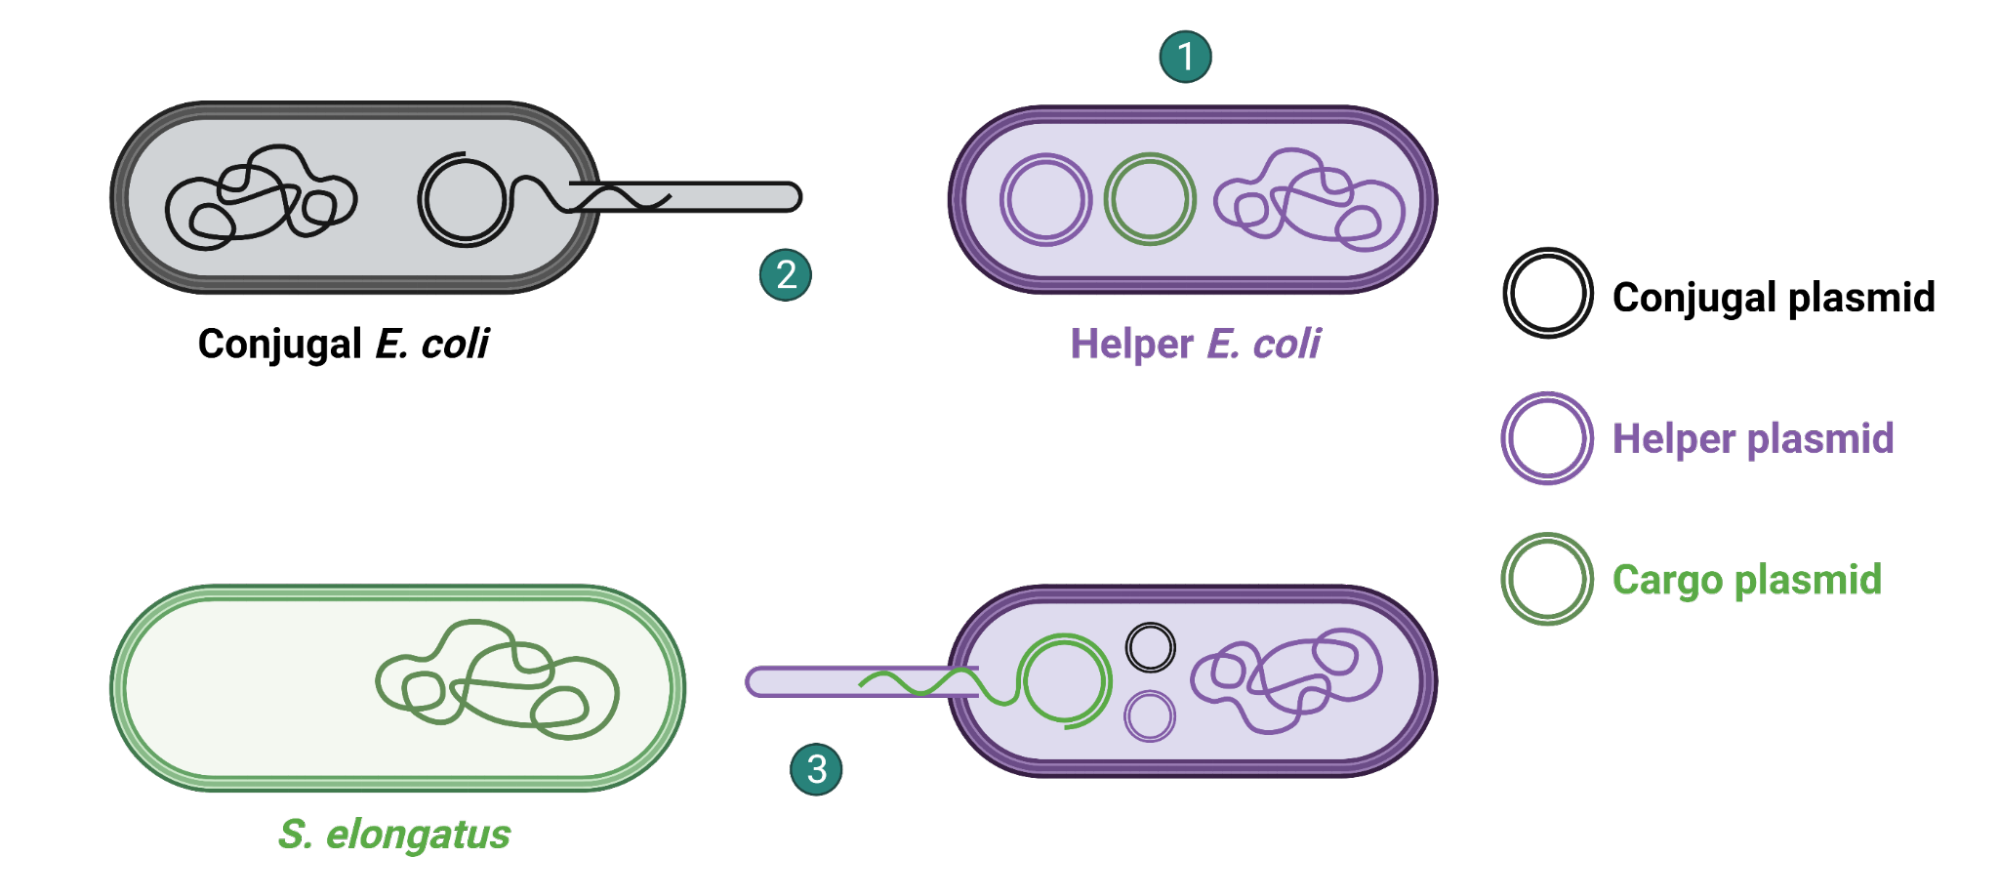
\includegraphics[width=\textwidth]{images/chap3/cyano/image1.png}
    \label{fig:ch3cyano01}
    \caption{Transfer of DNA into a cyanobacterium (green) through triparental mating (iGEM Toulouse 2021).} 
\end{figure}
\FloatBarrier

\noindent
There are several different conjugal and helper plasmids available, the most widely used in cyanobacterial research being respectively pRL443 (\href{https://www.addgene.org/70261/}{https://www.addgene.org/70261/}) and pRL623 (\href{https://www.addgene.org/58494/}{https://www.addgene.org/58494/}). The E. coli HB101 strain is furthermore frequently used for this type of protocol. More information on the practical protocol details can be found in the well-illustrated video article provided by \parencite{Gale2019}.
Overall, although theoretically the triparental mating process may seem complicated, in practice it is quite easy to perform and provides satisfactory transformation efficiencies for most applications. This technique is widely applied for species and strains that are not naturally competent. In some instances, conjugation may furthermore be the preferred route of DNA transfer, particularly when a large segment of foreign DNA is to be transferred or if merodiploids (single recombination events) are desired \parencite{Yu2015}. Note that certain species are refractory to conjugation, maybe due to thick cell walls or strong endonuclease activities.



\subsection{Electroporation}

Electroporation is the process of transferring DNA into bacteria or other cells by momentarily opening the pores of cell membranes with a pulse of electricity. A few species of cyanobacteria have been shown to be transformable by electroporation in laboratory conditions \parencite{Koksharova2002} \parencite{Stucken2012} \parencite{Tsujimoto2015}. \\ \\
If the strain of interest is not naturally competent and conjugation is impossible (some cyanobacteria - specific genetic sequences are toxic to E. coli), this method may be of interest \parencite{Wendt2019}. \\ \\
Nonetheless, in cyanobacteria, electroporation transformation has limitations. Earlier research has revealed that electroporation is inefficient and requires a considerable amount of donor DNA \parencite{Toyomizu2001}. Furthermore, the extracellular polysaccharide layers found in some cyanobacteria species cells act as physical barriers to DNA entering the cell \parencite{Wendt2019}. Moreover, electroporation may generate double strand DNA breaks within the cyanobacterial host genome and induce some undesired mutations.





\section{Higher Plants}
\epigraph{The following sections were written by Julia Macholl}{\textit{iGEM Bielefeld-CeBiTec 2021}}
\subsection{Overview}
There are many different techniques to transform plant or plant tissues that can be mainly separated into two big categories: Plants can be either transformed directly or indirectly, meaning that either the plant or plant tissue is directly transformed by physical or chemical methods or indirectly by using a biological host for the gene transfer. Many laboratories use either agrobacterium mediated transformation or particle bombardment due to practicality, simplicity, and efficiency \parencite{Keshavareddy2018}. 


\subsection{Indirect Methods}
The most common indirect method to transform plants or single plant cells is agrobacterium-mediated transformation \parencite{Hwang2017}. The soil bacterium \textit{Agrobacterium tumefaciens} has the natural ability to transform many dicot and monocot angiosperm as well as gymnosperm plants by incorporating T-DNA into the host genome \parencite{Gelwin2003}. For that, it carries a tumor inducing (Ti) plasmid that contains the T-DNA and vir genes that are, besides others, necessary to integrate the T-DNA into the plant genome. To transform plants, a binary vector system is used. The first vector contains the gene of interest that is flanked by T-DNA borders so that it will be incorporated into the plant genome. It also contains other important features like selection markers and origins of replication. The second vector – the Ti-helper plasmid – is carrying the vir-genes \parencite{Lee2008}.
\\

\begin{figure}[!htbp]
    \centering
    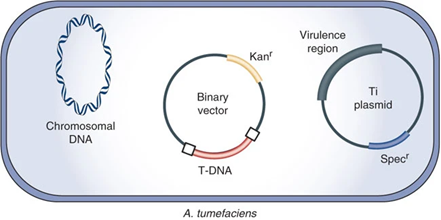
\includegraphics[width=\textwidth]{images/chap3/higher plants/image1.png}
    \label{fig:ch3high01}
    \caption{\textit{Agrobacterium tumefaciens} containing its chromosomal DNA, the Ti-helper plasmid and the binary vector \parencite{Michielse2008}.} 
\end{figure}
\FloatBarrier

\noindent
Transformation targets can either be tissue cultures or whole plants. (Stable transformation can be achieved with tissue cultures or whole plants.) For tissue cultures, plant cells are co-cultivated with agrobacteria for transformation \parencite{Keshavareddy2018}. Then, cells are cultured on media for formation of calli, which are unorganized plant cell mass. Calli can also be grown to whole transgenic plants in the end, which takes quite a long time.
Whole plants can also be transformed by several methods that were developed over time. One of the earliest methods developed was transformation by vacuum infiltration which can be performed not only on \textit{Arabidopsis} \parencite{Clough1998}, but also on other plants like Brassica campestris or Raphanus sativus. However, this method is quite labor intensive \parencite{Keshavareddy2018}. That is why it was replaced by more efficient techniques like floral dipping, where the flowers are dipped into agrobacterium suspension or floral spraying, where the agrobacterium suspension is sprayed onto the flowers. The advantage of in planta transformation in comparison to cell tissue transformation is that the gene of interest can be directly transferred into reproductive plants \parencite{Keshavareddy2018}.
\\
Besides stable transformation, transient expression of genes is also possible. The most prominent example is agroinfiltration with \textit{Nicotiana benthamiana}. For that, agrobacteria are injected into the underside of the leaf when the tobacco plants are ideally 4-6 weeks old. Two days after infiltration, the gene of interest should be expressed and experiments can be performed. Agroinfiltration is an easy method for screening constructs very quickly \parencite{Bally2018}. In comparison to stable transformation, which can take months or even up to years, transient expression with agroinfiltration allows quick screening in just a few days. 

\begin{figure}[!htbp]
    \centering
    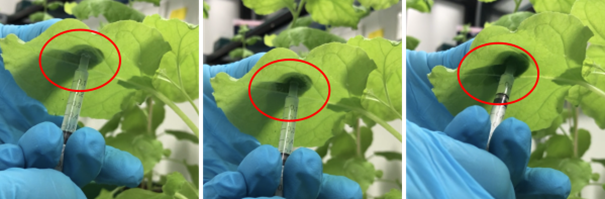
\includegraphics[width=\textwidth]{images/chap3/higher plants/image2.png}
    \label{fig:ch3high02}
    \caption{\textit{Agrobacterium} suspension is injected into the leaf with a needleless syringe.} 
\end{figure}
\FloatBarrier



\subsection{Direct Methods}
\epigraph{The following section was written by Jessica Baumann}{\textit{iGEM 
Marburg 2021}}
\noindent
Besides the indirect methods of transforming higher plants, there is also the direct method of biolistic bombardment. Biolistic bombardment is a process in which a gene construct is fired into plant cells using a particle gun. In this process, DNA is coupled to either gold or tungsten particles and is then catapulted into selected leaves under high pressure. 
This introduces the inserted DNA into the DNA of the chloroplast by homologous recombination. After successful insertion of the DNA, selection by antibiotics occurs, allowing only the transgenic plant cells to regenerate. First, it is important that the plants used for transformation grow sterile. For this purpose, at the beginning the seeds of the selected plants are sterilized by bleach and hydrochloric acid, and are then transferred to plant regeneration medium in deep petri dishes, where they begin to germinate. When the plantlets have reached a size of 1 cm, they are transferred to new petri dishes, where they continue to grow in fresh Plant regeneration medium. After a further growth phase, the plants are transferred to magenta boxes containing plant maintenance medium. The plants are grown in the magenta boxes until they reach a size of ~10 cm. Once the plants have reached this height, the biolistic bombardment can begin. 
\\ \\
For this purpose, the gold or tungsten particles are first prepared by repeatedly washing them with ethanol in several steps. For this purpose, the gold or tungsten particles are first prepared by repeatedly washing them with ethanol in several steps. To coat the Dna onto the particles, it is added to the particles while they are shaken on the vortex. After several more rounds of centrifugation, the particles are ready for the bombardment. First, however, the individual leaves of the sterile plants must be prepared for bombardment. For this purpose, 2 Whatman filter papers are applied to petridishes containing RMOP medium. The leaves previously harvested from the plantlets are placed centrally on the filters. It is important to sterilize the inner surfaces of the particle gun, as well as all other objects to be used, such as rupture disks or macrocarriers, etc., with ethanol. The DNA-coated particles are pipetted onto the macrocarriers. All individual components of the particle gun are assembled and the plates containing the sheets to be coated are placed one by one under the microcarrier launch assembly. Due to the pressure caused by the helium, the gold particles are bombarded into the plant cells. The bombarded plates are closed and sealed with micropore tape. Leaves are incubated in the Petri dishes for 2 days in a Culture room before leaf samples are transferred to additional plates containing a specific antibiotic. Several laef samples with a size of 1cm\textsuperscript{2} are cut out and transferred onto the antibiotic plates. These plates are also sealed with Micropore tape and again placed in the culture room. 6 to 12 weeks the leaf samples are kept on the medium until green calli or shoots are then formed. When spectomycin is used as an antibiotic, it can also happen that a spontaneous mutation in the 16S rRNA leads to resistance to the spectomycin just named. It remains to be determined which cells are truly transplastomic. If spectomycin is used for selection, small sections of calli or leaves are transferred to plates containing nict only spectinomycin but also streptomycin. The spontaneous mutation only introduces resistance to spectinomycin, but not to streptomycin. Thus, only transplastome cells remain. Whether the transgenes have really been inserted still has to be tested by PCR and DNA gel blot analysis. Rerun the plant regeneration on the selective RMOP medium and.
Validate the consistent transformation of the ptDNA by gel blot analysis. The transformed plants are then planted in soil and remain there until seeds are formed. These are collected and germinated again on antibiotic-containing plant maintenance medium. The transformed seedlings will appear dark green. 




\begin{figure}[!htbp]
    \centering
    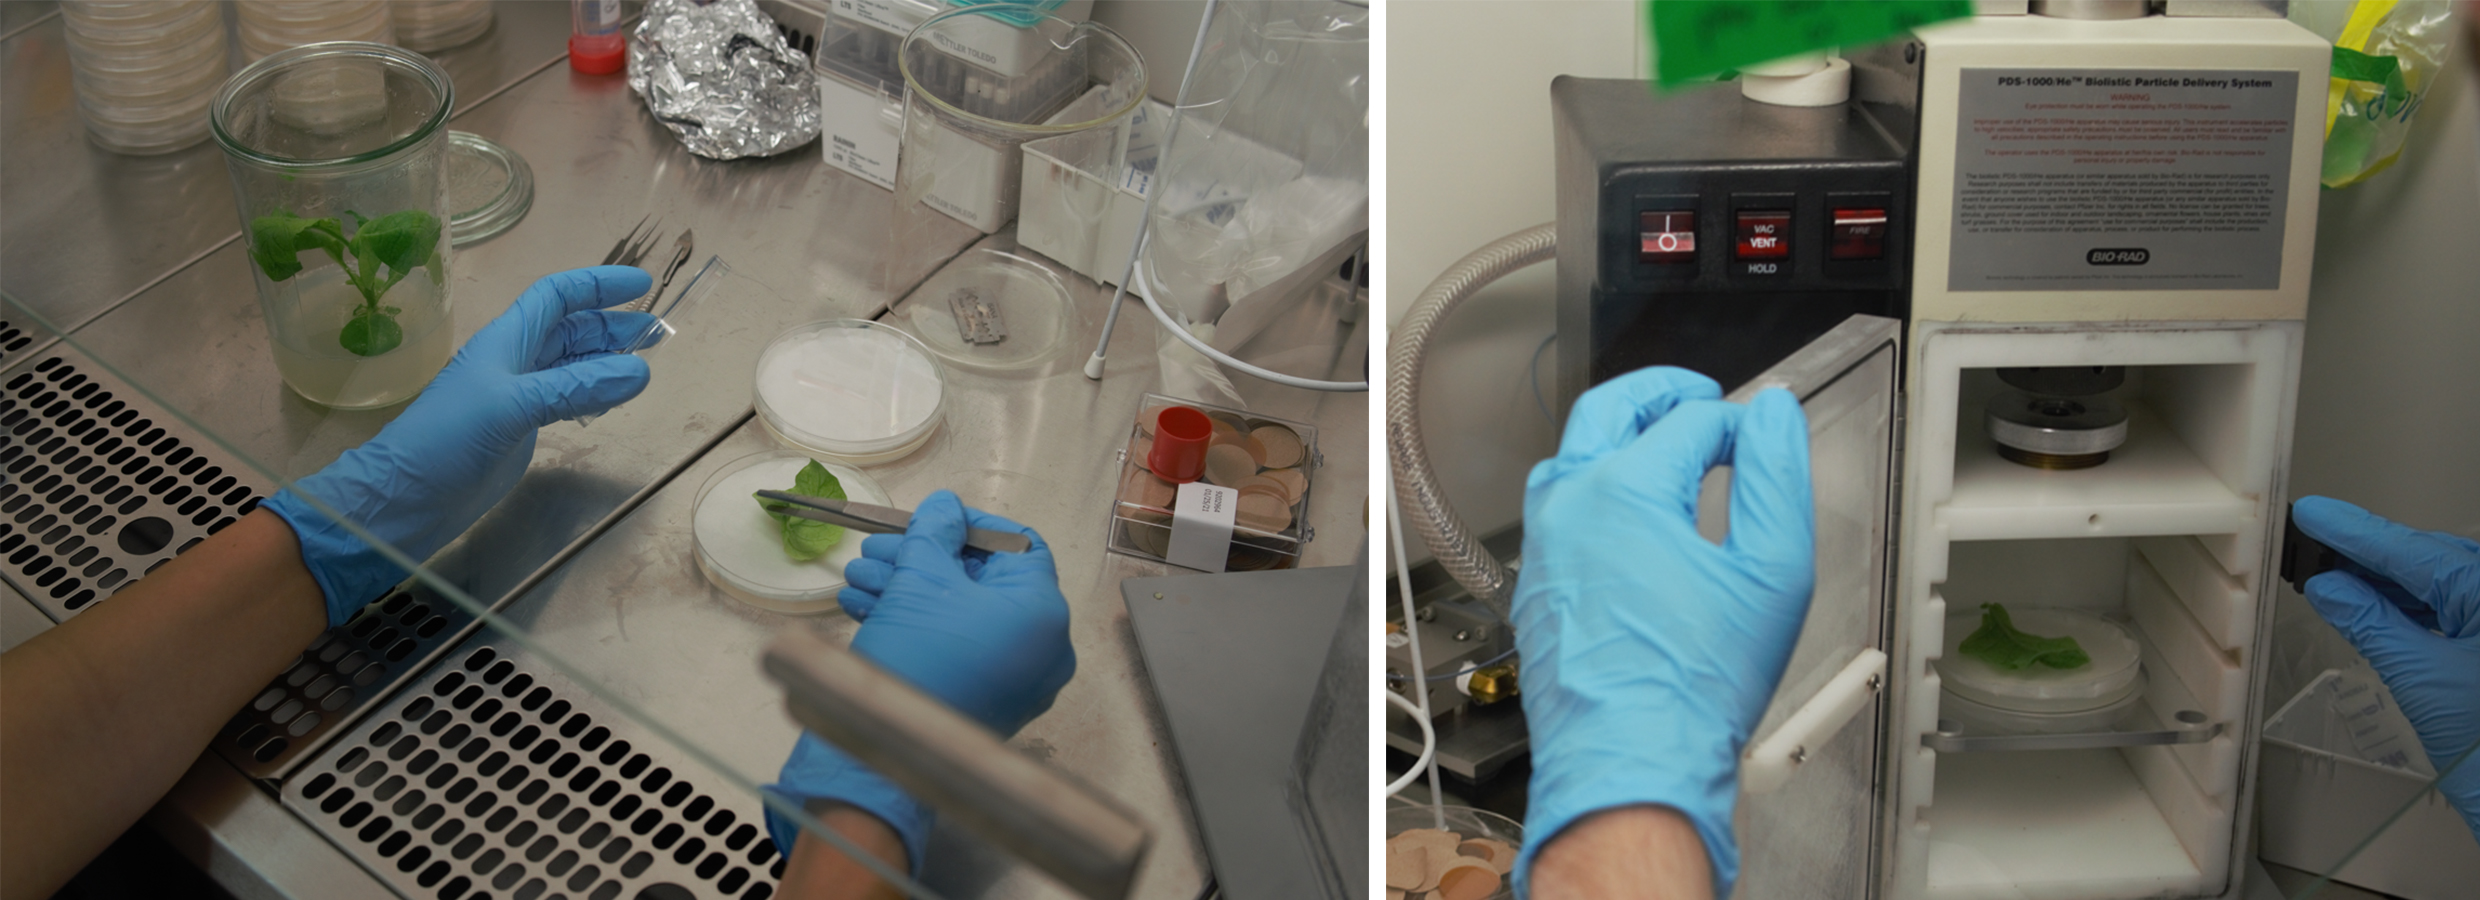
\includegraphics[width=\textwidth]{images/chap3/higher plants/image5.jpg}
    \label{fig:ch3high05}
    \caption{(a) Transfer of \textit{Nicotiana tabacum} leaves before bombardment with the gene gun. (b) The same leaf in the gene gun directly before introduction of a transgene.} 
\end{figure}
\FloatBarrier

\pagebreak

\section{Algae}
\epigraph{The following sections were written by members of the Sorbonne team}{\textit{iGEM Sorbonne\_U\_Paris 2021}}

\subsection{Overview}

The introduction of DNA into an organism allows the creation of de novo functions. This foreign DNA carry genes that usually code for a protein that provides this new function or a protein that is an intermediary to a compound that provides this function. Many of the epitomes of biotechnology are based on this principle. One notable example is the Golden rice, a rice variety that expresses components of the Β carotene pathway. This rice was engineered to improve the levels of vitamin A precursor to combat malnutrition worldwide.
\\ \\
The introduction of genetic material is not as straightforward as it may sound. Algae, as other organisms, have developed strategies to degrade foreign DNA that enters their cells. They developed these strategies because humans are not the first in the history of life that try to interfere with the genetics of algae. Viruses and bacteria, but also moving genetic elements, have interfered with the genomic cellular homeostasis since shortly after the emergence of first life. In order to defend themselves, organisms form barriers in the form of membranes and cell walls and target foreign DNAs and RNAs. Furthermore, genomic instability may also lead to apoptosis. The same system may target foreign genetic material integrating into the genome. Finally, the amount of chromosomes influences the effectiveness of transferring desirable functions: diploid and tetraploid species are more resistant than species that harbour only one chromosome of each kind. 
\\ \\
To overcome these challenges, scientists have developed direct and indirect methods to introduce novel genes into cells. Direct methods rely on challenging the outer barriers, such as membranes, through mechanical, electrical, and chemical methods. Indirect methods involve the hijacking of an existing pathological system that introduces genetic material into hosts. Both know their advantages and their challenges, which we review here.

\subsection{Indirect Methods}
Changing genomes through the transformation of a different species may be an avenue to pursue in certain cases. In this approach, we employ conjugative bacteria to do the job for us. The most famous example is \textit{Agrobacterium tumefaciens} while \textit{Escherichia coli} is also capable of transforming some algae \parencite{Mosey2021}. The choice for a direct or an indirect approach firstly depends on genome that is targeted, i.e. the nuclear genome in indirect approaches. Secondly, one has to realise that one major downside of the use of conjugative bacteria is that it takes more time and requires more steps. Moreover, one will first have to successfully transform the vector, verify that transformation, coculture and invite the conjugation to occur. Only then can we start to verify the transformation and characterisation of our newly transformed algae. This process can, however, be worthwhile in difficult to access nuclear genomes or when the insert is rather large: large inserts tend to be more prone to damage by nucleases in direct cloning methods.

\subsubsection{Indirect transformation through \textit{A. tumefaciens}}
In nature, \textit{A. tumefaciens} responds to phenolic compounds in wounds of plants through the virulence genes \parencite{Gelvin2017}. These conditions have to be reproduced to efficiently transform algae with A. tumefaciens. First of all, this means that coculture of algae not only with A. tumefaciens, but also plant cells may prove advantageous. Second and most important for effective transformation is the use of a phenolic compound. This can either be acetosyringone, cinnamic acid, vanillin or coumarin \parencite{Mosey2021}. The potential of this technique in algae was demonstrated early on in \textit{Chlamydomoas reinhardtii}. Moseley and others show a comprehensive overview of the transformation of non model microalgae (Figure 3.5). Pratheesh. Vineetha, and Muraleedhara Kurup provide a comprehensive protocol for the transformation of \textit{C. reinhardtii} using agrobacterium. For a comparison between direct and indirect transformation in \textit{C. reinhardtii} find Mini and others \parencite{Pratheesh2013}.

\subsubsection{Indirect transformation through \textit{E. coli}}
Three algae species have been reported to be succesfully transformed with \textit{E. coli}: \textit{S. obliquus}, \textit{N. oleoabundans}, and \textit{P. tricornutum} \parencite{Mosey2021} \parencite{Sharma2018} \parencite{George2020} \parencite{Beratto-Ramos2018} \parencite{Karas2015}. Important factors in the success of these transformations are the time and the ratio of the algae and the bacteria.


\begin{figure}[!htbp]
    \centering
    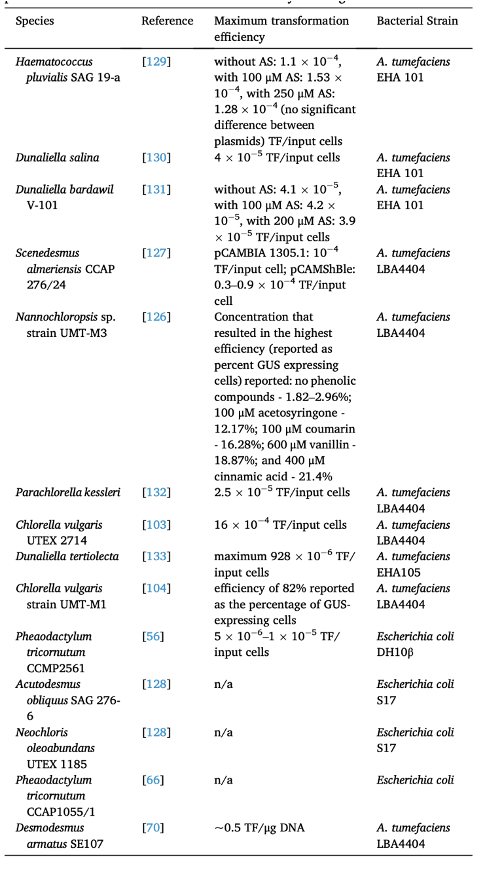
\includegraphics[width=0.8\textwidth]{images/chap3/algae/image1.png}
    \label{fig:ch3algae01}
    \caption{conditions for indirect transformations in non model microalgae \parencite{Mosey2021}.} 
\end{figure}
\FloatBarrier



\subsection{Direct Methods}
\epigraph{The following section was written by members of the Arizona State University team}{\textit{iGEM ASU 2021}}
\noindent
Our ASU iGEM 2021 team employed two direct methods of transformation into the chloroplast of the microalgae \textit{Chlamydomonas reinhardtii}. The two methods are biolistic bombardment with tungsten particles and agitation with glass beads. Most of our success this year was from our second attempt using biolistic bombardment. These two protocols were conducted under the direction of Dr. Kevin Redding, and the protocols were adapted from \parencite{Boynton1988} and \parencite{Wannathong2016} The algae used in the experiments came from the \href{https://www.chlamycollection.org/} {\textit{Chlamydomonas} Resource Center}. The sequence for the plasmid backbone used in these experiments, known as pASapI, was taken from the Wannathong paper as well \parencite{Wannathong2016}. The purpose of this section is to outline some of the tips and tricks our team learned during our time transforming the algae using these methods to help future iGEM students. The complete protocol can be found in the appendix, with some relevant notes. 


\subsubsection{Biolistic Bombardment}
Biolistic bombardment is a direct method of plasmid integration into the chloroplast. This process requires high-velocity microprojectiles made of either tungsten or gold and can utilize algae that has a cell wall (we used CC-4388). Therefore, this protocol is ideal because the resultant transformants will be easier to work with. Our experiment was conducted with 0.5 \textmu m tungsten particles in a gene gun made by Dr. Redding a few years ago (see Figure 3.6). The tungsten particles were first resuspended in glycerol, and coated in our plasmid by resuspending the DNA and the tungsten solution with calcium dichloride and spermidine. During this process, it’s important to ensure that the tungsten has not fallen out of solution and that there is never a high concentration area of spermidine, as that will lead to clumping of the tungsten/DNA. Ensure that the spermidine is added last, and the tube is being vortexed while it is added (takes practice!). Additionally, to ensure that the tungsten has not settled out of solution before placing it on the filter, the DNA solution should be sonicated thoroughly right before it is added to the filter and shot onto the plate coated in algae. This is a tedious, but important step, and make sure not to forget ear protection while sonicating! Once the filter has been loaded and screwed into the top of the chamber, ensure that the top of the agar is 11 cm from the tip of the filter. This ensures that the particle bombardment will be the correct size. The algae directly in the area of bombardment will die, and the algae near the edges of that area will survive with the plasmid integrated. Therefore, the area of bombardment should be centered on the plate, and should not occupy the whole space. In order to shoot the particles at the plate at a high enough velocity, the gene gun must create a vacuum. In our gene gun (Figure 3.6) the yellow lid sits on a rubber ring to allow the chamber to create a vacuum. Always ensure that the lid will form a complete seal before engaging the vacuum and shooting the algae. Once the bombardment has been delivered, you can see the area that was hit with the particles by holding the plate up to the light. While the rest of the agar should be clear, the area hit with the tungsten particles will appear a little hazy or fuzzy. There should not be visible dark clumps of tungsten particles. This indicates that the solution was not sonicated properly or distributed on the filter improperly. 
\\ \\
Both of these protocols utilize photosystem II deficient \textit{C. reinhardtii} and restore function of the photosystem with the plasmid. This means that photosynthesis is restored when the plasmid is integrated into the chloroplast genome. Therefore, the plates need to be stored in the light to allow for the selective selection of the transformed colonies. That being said, we initially had no success with our first round of shooting \textit{C. reinhardtii}. It was then suggested to us by our friends in Marburg that we store the algae in the dark for 24 hours before exposing it to the light. We added this step to our protocols for the second round of shooting. This time, we exposed half of the plates to the dark for 24 hours before putting them in the light and put half of the plates in the light immediately. This round of shooting was successful, but only marginally. After 4 weeks, one colony was found on three different plates, out of ~30 plates. Two of the successful plates were put directly in the light, and one of the plates was placed in the dark for 24 hours. At this point, we cannot recommend whether the light or dark protocol is more successful. 
\\ \\
Overall, we recommend a few things. First, shoot at least four different plates with the same construct. Second, ensure that the reagents used to make the tungsten/DNA solution are fresh and get mixed thoroughly. Third, double parafilm the plates before leaving them under the light to ensure no contaminants get in. Fourth, start this process EARLY. The three colonies we found were only visible one month after shooting. Finally, this process does take practice, so budget your time for multiple iterations. 

\begin{figure}[!htbp]
    \centering
    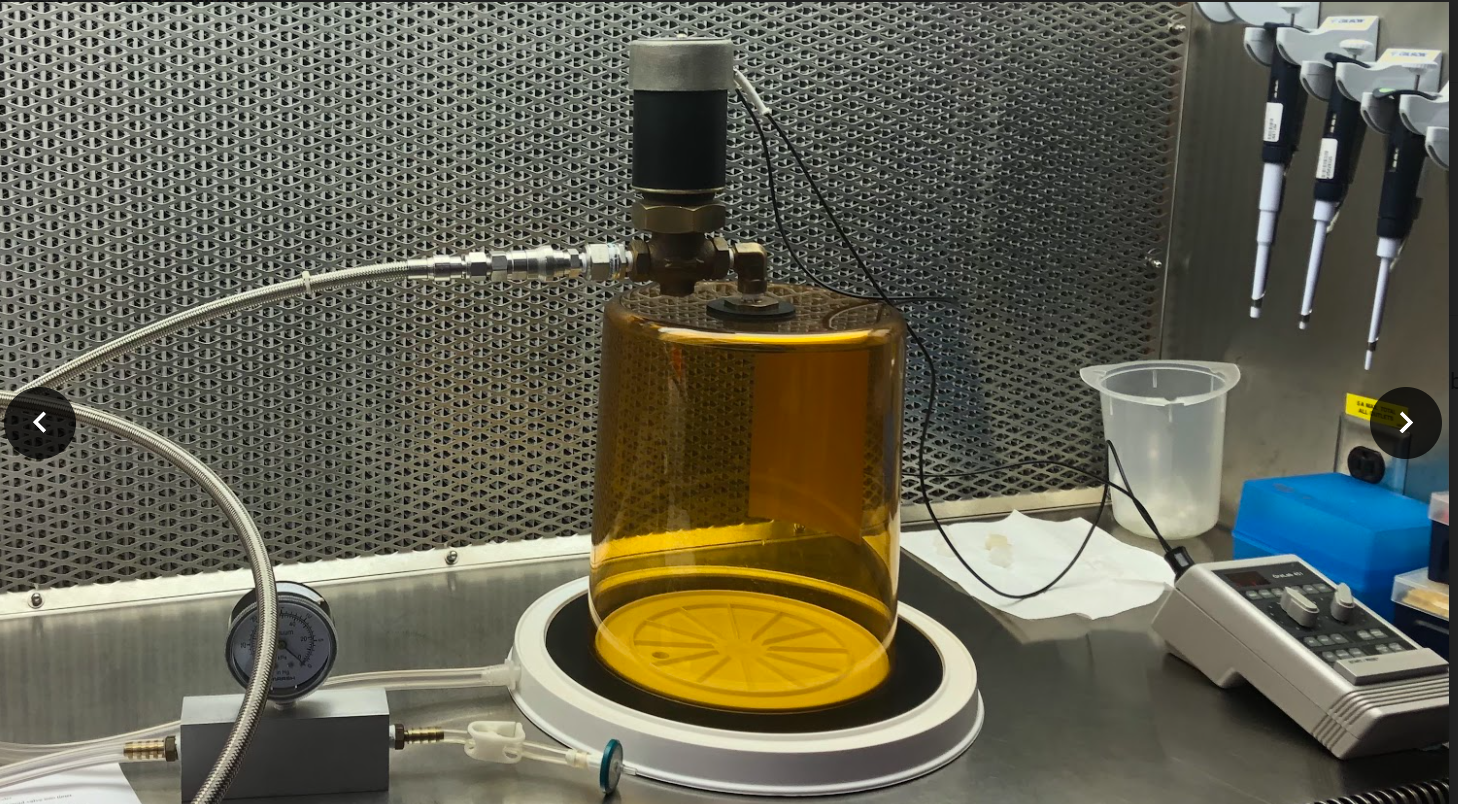
\includegraphics[width=\textwidth]{images/chap3/algae/image2.png}
    \label{fig:ch3algae02}
    \caption{The gene gun, created by Dr. Redding, set up in a laminar flow hood. On the right, the timer and button to release Helium. In the center, the yellow lid of the chamber. (Not pictured, a lab jack used to move the plate up 11 cm away from the tip of the filter).} 
\end{figure}
\FloatBarrier



\begin{figure}[!htbp]
    \centering
    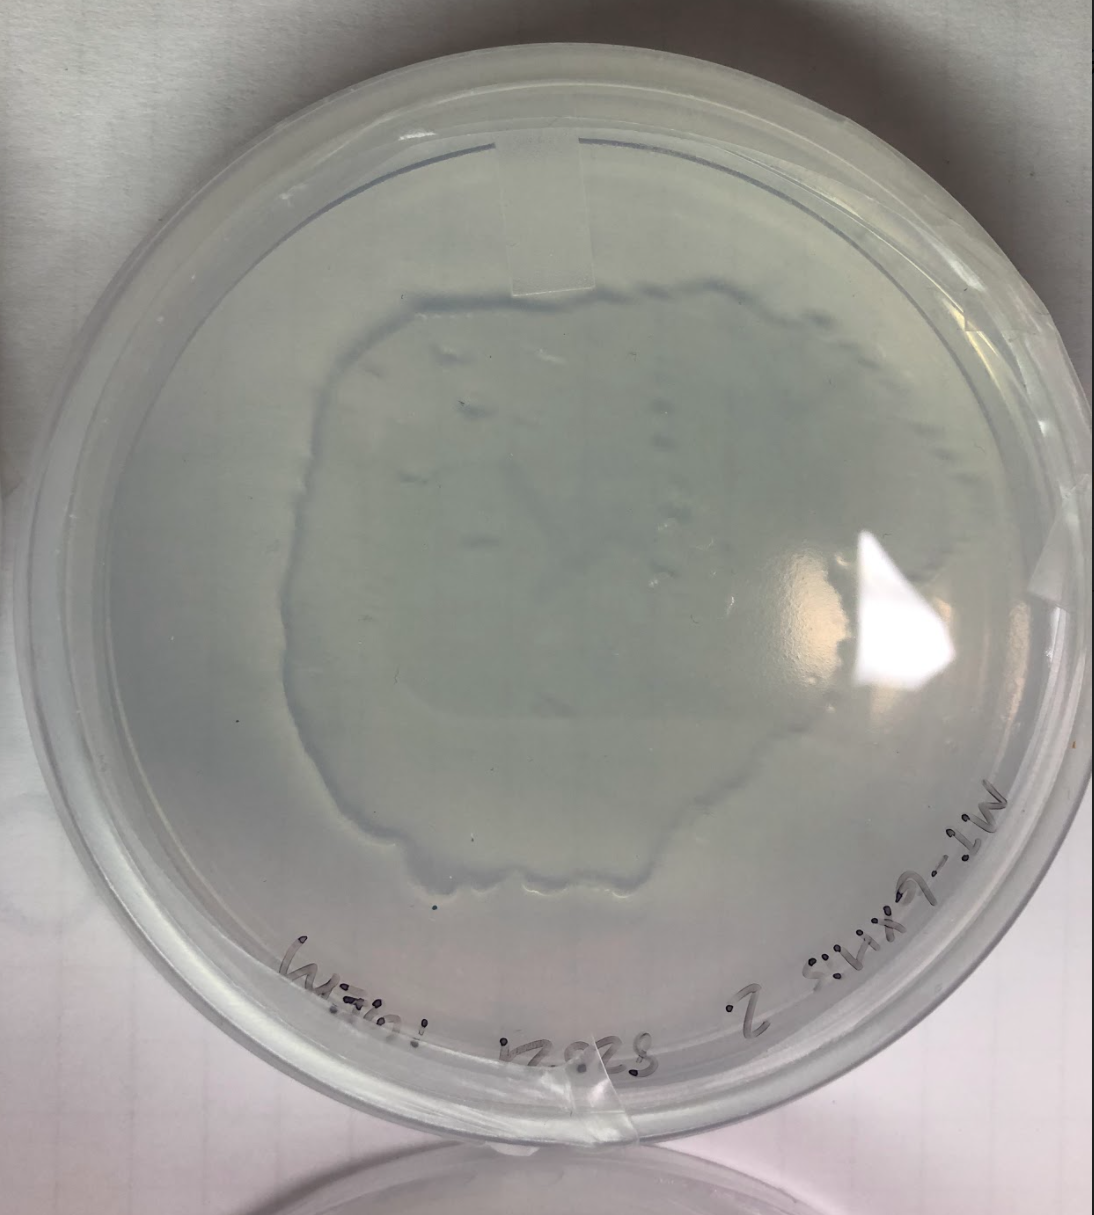
\includegraphics[width=0.7\textwidth]{images/chap3/algae/image4.png}
    \label{fig:ch3algae04}
    \caption{One of the plates with a transformed colony, creating the strain now known as iGEMC3. TBP plate, CC-4388 transformed with pASapI/MT-6xHIS. The small dark spot seen approx 0.5 cm below the “iGEM” is the successful colony. The ride that is seen at the center of the plate is water that has amassed on the lid of the plate due to condensation. It is not touching the agar of the plate and has no effect on the algae.} 
\end{figure}
\FloatBarrier




\subsubsection{Glass Bead Agitation}
Glass bead agitation is a means of integrating a plasmid into the chloroplast of \textit{C. reinhardtii}. However, this process is not ideal because it requires the use of cell wall deficient microalgae (we used CC-5168), which makes the transformant more difficult to work with. This protocol, taken from \parencite{Wannathong2016} has not yet yielded any transformants, after a full month of incubation in the light. However, it comes from a reputable source, and we had not attempted this protocol before, so it is most likely a mistake on our part. This protocol utilized cell wall and photosystem II deficient \textit{C. reinhardtii}, and the same plasmids as used in the gene gun protocol. Because our team only performed this protocol once, we do not have as many recommendations for successful transformation. 
	To make the best use of the time, it is best to aliquot out the 400-624 um diameter beads into the test tubes a day or two ahead of time, and autoclave them to ensure they are sterile. Additionally, the top agar should always be stored in a warm water bath, and should not be allowed to congeal: it should be alliquoted day of in to ~6ml samples. We plated the cells on both HSM and TBP plates, with 5\% top agar used for both plates. This protocol calls for a lot of DNA (5-10$\mu$g) in a small concentration (not more than 50$\mu$L). In order to get this concentrated DNA, we performed a miniprep on 5mL of culture and eluted the DNA thoroughly from the column. During the glass bead protocol, ensure that the vortex is at top speed, and that it runs for a full 15 seconds(Figure 3.8). Then, when removing the cells from the tube, ensure there are no glass beads clinging to the pipette tip. When mixing the cells into the top agar, invert gently and spread on the plates as evenly as possible. Ensure the top agar has congealed completely before being stored in the light. Should the colonies arise, they may be embedded in the top agar. This simply means that you’ll need to go digging for them to use the transformants. 
	Overall, we were not as successful with this protocol as we were with the gene gun. We recommend starting an assembly line of sorts with multiple lab members to work most efficiently. The algae should be removed from the glass beads, added to the top agar, and plated quickly after agitation. Additionally, the top agar should never be allowed to congeal before it is plated, and should only be removed from the warm water bath right before the algae is added. 


\begin{figure}[!htbp]
    \centering
    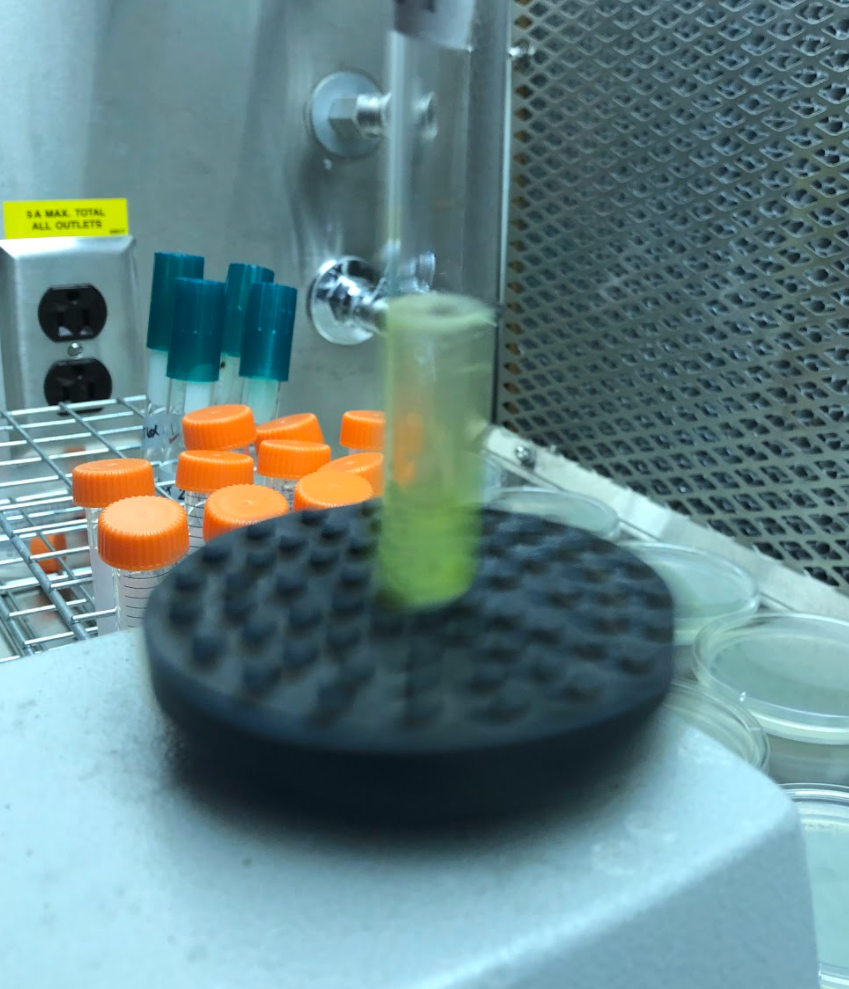
\includegraphics[width=0.8\textwidth]{images/chap3/algae/image3.png}
    \label{fig:ch3algae03}
    \caption{Test tube containing glass beads, \textit{C. reinhardtii} CC-5168, and DNA being agitated on the vortexer at max speed in the laminar flow hood.} 
\end{figure}
\FloatBarrier